\documentclass[a4paper]{report}
\usepackage{times}
\usepackage[utf8]{inputenc}
\usepackage[pdftex]{graphicx}
\usepackage{multicol}

% to customize headers and footers
\usepackage{fancyhdr}
\pagestyle{fancy}
\chead{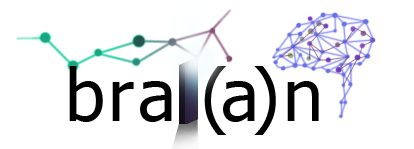
\includegraphics[scale=0.2]{braian} \vspace{50cm}}
\rfoot{\vspace{1cm} 
\includegraphics[scale=0.03]{Logo-Epitech}}

\newcommand{\HRule}{\rule{\linewidth}{0.5mm}}

\begin{document}
  \begin{titlepage}
  \begin{center}

    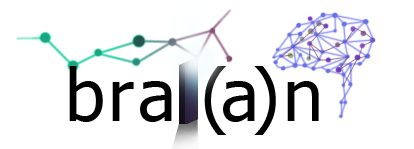
\includegraphics[width=0.7\textwidth]{braian}~\\[1cm]

    \textsc{\LARGE Epitech Paris}\\[1.5cm]

    \textsc{\Large Fiche Projet - PFA}\\[0.5cm]

    % Title
    \HRule \\[0.4cm]
    { \huge \bfseries Brai(a)n - An AI who learns \\[0.4cm] }

    \HRule \\[1.5cm]

    \noindent

    \begin{multicols}{3}
      \emph{Chef Technique:}\\
      Sebastien \textsc{Maire} \\

      \vspace{1cm}

      \emph{Technique:} \\
      Alexandre \textsc{Fulgoni} \\

      \emph{Technique:} \\
      Stephane \textsc{Nguyen} \\

      \vspace{1cm}

      \emph{Manageur:} \\
      Thomas \textsc{Nieto} \\

      \vspace{1cm}

      \emph{Technique:} \\
      Emmanuel \textsc{Isidore} \\

      \vspace{1cm}

      \emph{Technique:} \\
      Thomas \textsc{Valentin} \\
   \end{multicols}

    \vfill

    {\large \today}

  \end{center}

  \begin{flushright}
    \vspace{1cm}
    
\includegraphics[scale=0.03]{Logo-Epitech}
  \end{flushright}

\end{titlepage}



  \section{Introduction}
    Au regard de ce que la science-fiction a imaginé dans le domaine de l'intelligence artificielle, l'informatique moderne n'en est qu'à ses balbutiements.
    Prenons quelques examples en littérature : HAL dans 2001, l'Odyssée de l'Espace ;
    en cinéma : JARVIS dans Iron-Man ou Terminator dans les film de mêmes noms ; ou encore dans le jeu-vidéo : Cortana dans HALO... Pour ne citer qu'eux. \\
    Le plus pertinant exemple d'IA qui nous accompagne ? Siri, une voix monotone dans un téléphone qui se décharge en dix heures...
    D'une part, nous avons des personnages qui ont une personnalité et d'autre part, un assistant électronique qui ressemble davantage à un easter egg qu'à une vraie fonctionnalité. \\

    \noindent
    La différence la plus flagrante entre ces IA et Siri ? Leur comportement. \\
    En effet, les IA de sciences-fictions ne sont pas imaginés avec un carcan intellectuel.
    Ces dernières évoluent, intéragissent, échangent, se remettent en question. Cela n'est permis qu'avec l'apprentissage. \\

    \noindent
    C'est sur ce dernier point, que nous avons décidé de travailler. \\
    Nous nous concentrerons alors, sur l'aspect apprentissage et la prise de décision d'une intelligence artificielle.

    % Le domaine de l'intelligence artificielle étant vaste et complexe.
    % Environnement Minecraft - Terraria - Spelunky

  \section{Equipe}
    \begin{description}
      \item[Sébastien Maire] \hfill \\
        \textbf{Chef Technique} \\
        Motivé par l'application de ses connaîssances en algorithmie et leur approndissement
      \item[Alexandre Fulgoni] \hfill \\
        \textbf{technique} \\
        A toujours été motivé par l'IA et leur domaine d'application.
      \item[Stéphane Nguyen] \hfill \\
        \textbf{technique} \\
        intéressé par le développement de jeu-vidéo. En effet,
        au-delà du graphisme, l’IA est LE pillier qui permet le réalisme
        et donc l’immersion du joueur.
      \item[Thomas Nieto] \hfill \\
        \textbf{Recherche et managment} \\
        L'apprentissage en IA est un peu \textit{terra igognita}. Thomas a un âme d'explorateur.
    \end{description}

    \noindent
    Première fois ensemble dans un groupe. Nous nous sommes rencontrés grâce aux
    intérêts que nous partageons et sommes donc tous motivés pour aller le plus
    loin possible.

  \section{Contexte}
    Brai(a)n n'existe que dans un contexte de recherche. Aucune application ou produit
    n'est prévu. De plus, il s'agit d'un projet Open Source, nous espérons voir d'autres personnes prendre part à l'aventure.

    
    Utilisation d’algorithmmes d’apprentissage et application dans un monde
    virtuelle pour la démo pour nous : Apprentissage / découverte et
    application de l’IA

  \section{Partenaire}
    L'Epitech Innovation HUB

  \section{Objectifs}
    Coupler prise de décision et apprentissage
    Cas concret : arbre de décision qui change ses nodes.


  \section{Planning}
    2 jours par semaine : Samedi et dimanchehey


\end{document}
% # Introduction
%% Le but de ce pfa est de réaliser une intelligence artificielle.
%
% <AI étant vaste, nous nous concentrons sur l’apprentissage>
% Notre projet se concentrera sur l’aspect apprentissage et prise de décision.
%
%
% Environnement Minecraft - Terraria - Spelunky

%
% # Equipe
% * Sebastien Maire
%     * chef technique
%     * appliquer des connaissances en algorithmie et les approfondir
%     grace à un cas concret qu’est ce pfa
% * Alexandre Fulgoni
%     * technique
%     * l’IA a toujours été un domaine vers lequel a toujours voulu travailler dans l’IA, ce pfa s’est tout naturellement posé
% * Stephane Nguyen
%     * technique
%     * intéressé par le développement de jeu-vidéo. En effet, au-delà du graphisme, l’IA est LE pillier qui permet le réalisme et donc l’immersion du joueur.
% * Thomas Nieto
%     * recherche et manager d’equipe
%     * ...
%
% Première fois ensemble dans un groupe. Nous nous sommes rencontrés grâce aux intérêts que nous partageons et sommes donc tous motivés pour aller le plus loin possible.
%
%
% # Contexte
% Ce projet n’a pas pour vocation d’être distribué à des fins commerciales. C’est purement un
% projet de R&D en partenariat avec le HUB.
% Utilisation d’algorithmmes d’apprentissage et application dans un monde virtuelle pour la démo
% pour nous : Apprentissage / découverte et application de l’IA
%
% # Partenaire
% HUB
%
% # Objectifs
% Coupler prise de décision et apprentissage
% Cas concret : arbre de décision qui change ses nodes.
%
% # Planning général
% 2 jours par semaine : Samedi et dimanche
